\documentclass[a4paper, 11pt]{article}
% TeX-template
% Copyright (c) 2024 Joseph Tooby-Smith. All rights reserved.
% Released under Apache 2.0 license.
% Paper content: 
% Copyright (c) 2024 Joseph Tooby-Smith. All rights reserved.
\usepackage{xcolor}
\usepackage{setspace}

\onehalfspacing%
%\setstretch{3} % Custom separation of lines.
\renewcommand{\arraystretch}{1.5}
%%%%%%%%%%%%%%%%%%%%%%%%%%%%%%%%
%Hyperlinks
\usepackage{hyperref}
\definecolor{mycolor}{RGB}{0,88,204}
\hypersetup{
  colorlinks=true,
  linkcolor=mycolor,
  urlcolor=mycolor,
  citecolor=mycolor
}
%%%%%%%%%%%%%
%Watermark
\usepackage{draftwatermark}
\SetWatermarkText{\color{mycolor} DRAFT}
\SetWatermarkScale{1.5}
%%%%%%%%%%%%%%%%%%%%%%%%%%%%%%%%
%Mathematics
\usepackage{amsmath}
%%%%%%%%%%%%%%%%%%%%%%%%%%%%%%%%
%Margins
\usepackage{geometry}

\geometry{
  top=0.8in,
  bottom=0.8in,
  left=1in,
  right=1in
}
%%%%%%%%%%%%%%%%%%%%%%%%%%%%%%%%
%Page numbers
\usepackage{fancyhdr}


\pagestyle{fancy}
\fancyhf{}
\fancyhead[R]{\thepage}
\renewcommand{\headrulewidth}{0pt}
\setlength{\headheight}{13.6pt}
%For the title page
\fancypagestyle{plain}{%
  \fancyhf{}
  \fancyhead[R]{\thepage}
  \renewcommand{\headrulewidth}{0pt}
}
%%%%%%%%%%%%%%%%%%%%%%%%%%%%%%%%
%Fonts

\usepackage{mathptmx}

%%%%%%%%%%%%%%%%%%%%%%%%%%%%%%%%
%Section style

\usepackage{titlesec}

\titleformat{\section}
  {\normalfont\large\centering}{\thesection.}{1em}{\MakeUppercase}
\titleformat{\subsection}
  {\normalfont\centering}{\thesubsection.}{1em}{\MakeUppercase}

  \titlespacing{\paragraph}{10pt}{0pt}{6pt}[0pt]
%%%%%%%%%%%%%%%%%%%%%%%%%%%%%%%%
%Comments

\newcommand{\js}[1]{ {\color{magenta} js:  #1}}

%%%%%%%%%%%%%%%%%%%%%%%%%%%%%%%%
%SVG images
\usepackage{svg}
%%%%%%%%%%%%%%%%%%%%%%%%%%%%%%%%
%Paragraph markers
%\newcommand{\paragraphMarker}[1]{ %{\color{gray} $\langle$#1$\rangle$}
%}
%%%%%%%%%%%%%%%%%%%%%%%%%%%%%%%
%Lean formating
\usepackage{listings}
\usepackage[T1]{fontenc}
\usepackage[utf8]{inputenc}
\usepackage{amssymb}
\usepackage{chngcntr}
\definecolor{keywordcolor}{rgb}{0.7, 0.1, 0.1}   % red
\definecolor{tacticcolor}{rgb}{0.0, 0.1, 0.6}    % blue
\definecolor{commentcolor}{rgb}{0.4, 0.4, 0.4}   % grey
\definecolor{symbolcolor}{rgb}{0.0, 0.1, 0.6}    % blue
\definecolor{sortcolor}{rgb}{0.1, 0.5, 0.1}      % green
\definecolor{attributecolor}{rgb}{0.7, 0.1, 0.1} % red

\def\lstlanguagefiles{lstlean.tex}
\lstset{
 	frame = lrtb,
 	rulecolor=\color{mycolor},
	language=lean,
	aboveskip = 5mm,
	belowskip = 5mm,
	captionpos=t
	}

\lstnewenvironment{code}[1][]%
{
   \noindent\newline
   \minipage{\linewidth}
   \vspace{0.5\baselineskip}
   \lstset{
 	frame = lrtb,
 	rulecolor=\color{mycolor},
 	escapeinside={/*!}{!*/},
	language=lean,
	aboveskip = 5mm,
	belowskip = 5mm,
	xleftmargin=2mm,
	xrightmargin=2mm,
	}
	}
{\endminipage\newline}
\lstnewenvironment{codeLong}[1][]%
{
   \lstset{
 	frame = lrtb,
 	rulecolor=\color{mycolor},
 	escapeinside={/*!}{!*/},
	language=lean,
	aboveskip = 5mm,
	belowskip = 5mm,
	xleftmargin=2mm,
	xrightmargin=2mm,
	}
	}
{}
%%%%%%%%%%%%%%%%%%%%%%%%%%%%%%%%
%Links in code block
% put at top of code block using
% /*!\codeLink{...}!*/
\newcommand{\codeLink}[1]{
  \vspace{-0.5cm}\hfill\href{https://github.com/HEPLean/HepLean/blob/1b951994ae3d882242b02d23957ef1ee7fa05f3d/HepLean/#1}{(source)}
  }
  \newcommand{\codeBreakdownLink}[2]{
  \vspace{-0.5cm}\hfill\href{https://github.com/HEPLean/HepLean/blob/1b951994ae3d882242b02d23957ef1ee7fa05f3d/HepLean/#1}{(source)}
  (breakdown \ref{#2})
  }
 \newcommand{\textLink}[1]{\href{https://github.com/HEPLean/HepLean/blob/1b951994ae3d882242b02d23957ef1ee7fa05f3d/HepLean/#1}{source}}
 \newcommand{\textLinkB}[1]{\href{https://github.com/HEPLean/HepLean/blob/1b951994ae3d882242b02d23957ef1ee7fa05f3d/HepLean/#1}{(source)}}
%%%%%%%%%%%%%%%%%%%%%%%%%%%%%%%%
%Title, author, date
\title{Index notation in Lean 4}
\author{Joseph Tooby-Smith \\ \textit{Reykjavik University}}
\date{\today}
%%%%%%%%%%%%%%%%%%%%%%%%%%%%%%%%

\begin{document}
\counterwithin{lstlisting}{section}
\maketitle
\vspace{-1cm}
\begin{abstract}
Index notation is a tool commonly used in physics to manipulate tensors.
In physics, we use index notation for three different types of tensors: 
Einstein tensors (e.g., ordinary vectors and matrices), Lorentz tensors, and 
Van der Waerden tensors. In this paper, we discuss how these are implemented in Lean 4 using a 
general mathematical theory based on category theory, and related to the notation of an operad.
\end{abstract}

\section{Introduction}

A previous work by the current author, presented the first steps of digitalizing (or formalizing)
results from high energy physics into the interactive theorem prover Lean 4. This 
project is called HepLean. Lean is a programming language whose syntax looks similar to 
what we pen-and-paper mathematics, and is used to write and automatically check 
 statements of definitions and theorems, and proofs of theorems.
HepLean has four main motivations: \js{sorry}


When writing and proving results on paper, the physicists is accustumed to using notation, and no
notation abounds in physics more than index notation.
Thus as part of the larger HepLean project, index notation has been implemented by 
the author in to Lean 4.
Any such implementation must satisfy two basic requirements: 
\begin{enumerate}
  \item Must be mathematically rigourous. 
  \item Must be easy to use.
\end{enumerate} 
The first requirement is a consequence of Lean being a proof assistant, and not able to accept 
anything else but formally defined results. 
The second requirement is due to the fact that many other results will depend on the 
implementation of index notation. We beleive the implementation dicussed within this paper 
does satisfy both of these requirements.  





\begin{itemize}
\item Notational conventions abound in physics, and non-more so then index notation. 
\item Notation, in general, is a way for the writer to compactly write down a term in a 
  mathematical expression. The reader can implicitly unfold or elborate the compactly written term 
  back into its full underlying meaning. 
\item Index notation is a compact way of writing expressions involving tensors.
\item With tensors there is a notion of contraction, evaluation and permutation.
\item All of these notions can defined independently of index notation.
\item Index notation is a way of writing these operations in a compact way.
\item In a previous work by the current author, the first foray of formalizing high energy physics 
  in Lean 4 was undertaken, in a project called `HepLean'.
\item One aim of that project is to make Lean easier for the high-energy phsycisists to use. 
\item Motiviated by this aim, we have implemented index notation in Lean 4.
\item In this paper, we will discuss how this is done.
\item This is, of course, not the first paper dicussing the implmentation of index notation in a 
  programming language. However, Lean, being a proof assistant, has a different set of requirements. 
\item In particular, Lean has to be provided a proof of everything. 
\item We also believe that the underlying mathematics used to implement index notation here 
 is novel. 
\end{itemize}

\section{Implementation of index notation into Lean 4}
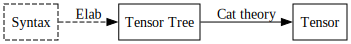
\includegraphics[width=\textwidth]{overviewFlow.png}


\section{Complex Lorentz Tensors}
There are three different species of tensors that physicists deal with: 
\begin{itemize} 
  \item Einstien tensors (i.e., ordinary vectors and matrices transforming under $SO(n)$)
  \item Real Lorentz tensors (i.e., tensors in a real vector space transforming under the Lorentz group)
  \item Complex Lorentz tensors (i.e., tensors in a complex vector space transforming under the $SL(2,\mathbb{C})$)
\end{itemize} 
In this paper, since it is the most complicated, we will use the complex Lorentz tensors as an example.

In a tensor species there are different kinds of indices. We shall call the different 
kinds of indices `colors'. For example, for complex Lorentz tensors there are six colors of indices.
In Lean we put these colors into an inductive type 
\begin{code}
inductive Color
  | upL : Color
  | downL : Color
  | upR : Color
  | downR : Color
  | up : Color
  | down : Color
\end{code}


\subsection{Symmetric and anti-symmetric tensor}

Let  $S_{\mu \nu}$ be complex Lorentz tensors where $\mu$ and $\nu$ are 
4-vector indices. The corresponding 
\begin{code}
(S : complexLorentzTensor.F.obj (OverColor.mk ![Color.down, Color.down]))
\end{code}

To explain this notation let us work from the right to the left.



\section{Future work}

\bibliographystyle{unsrturl}
\begin{spacing}{0.5}
\bibliography{MyBib}
\end{spacing}


%%%%%%%%%%%%%%
\end{document}
